\documentclass[10pt]{beamer}

\usetheme{CambridgeUS}
\usepackage[english, russian]{babel}
\usepackage[utf8]{inputenc}
\usepackage{caption}
\usepackage{etoolbox}
\usepackage{multicol}
\usepackage{listings}

\definecolor{mygreen}{rgb}{0,0.6,0}
\lstset{
  basicstyle=\ttfamily\footnotesize,        % the size of the fonts that are used for the code
  breaklines=true,                 % automatic line breaking only at whitespace
  captionpos=b,                    % sets the caption-position to bottom
  commentstyle=\color{mygreen},    % comment style
  keywordstyle=\color{blue},       % keyword style
  stringstyle=\color{red},     % string literal style
  showstringspaces=false,
  morekeywords={include, printf},
  texcl=true     %<---- added
}

\title[Ввдение в обработку естественных языков]{Морфемная сегменатция}
\author[Гусев Илья]{Гусев Илья}
\institute[МФТИ] 
{Московский физико-технический институт\\*}
\date{Москва, 2018}
\subject{Computer Science}

\begin{document}

\begin{frame}
  \titlepage
\end{frame}

\begin{frame}{Содержание}
\tableofcontents
\end{frame}

\section{Морфемная сегментация}

\subsection{Задача}
\begin{frame}[fragile]{Задача морфемной сегментации}
\begin{itemize}
    \item По слову нужно получить его разбиение на морфемы.\\
    \item Мотивация - обработка редких и не встретившихся в обучющей выборке слов для раличных задач NLP.\\
    \item Разбиение на морфемы можно использовать вместо BPE (byte pair encoding), морфемы обычно имеют какой-то смысл.
\end{itemize}
\end{frame}

\begin{frame}[fragile]{Отступление: byte pair encoding}
\begin{itemize}
    \item Считаем самую частотную пару символов одним символом
    \item Повторяем, пока все не будут встречаться по одному разу или пока за каждым символом < N терминалов
    \item Мотивация - сильно уменьшаем размер словаря по сравнению с word-level, но при этом это лучше, чем char-level в некоторых случаях
\end{itemize}
Пример:\\
\begin{enumerate}
    \item aaabdaaabac
    \item ZabdZabac
    \item ZYdZYac
    \item XdXac
\end{enumerate}
\end{frame}

\begin{frame}[fragile]{Задача морфемной сегментации}{Примеры}
\begin{center}
\begin{tabular}{ |c|c| } 
забытье & забы*ть*е \\
статичный & стат*ич*н*ый \\
учитель & уч*и*тель \\
скрыться & скры*ть*ся \\
тысячами & тысяч*ами \\
подержаться & по*держ*а*ть*ся \\
\end{tabular}
\end{center}
\end{frame}

\subsection{Morfessor}
\begin{frame}[fragile]{Morfessor}{Data likelihood 1}
$W$ - слова, $w \in W$ \\
$A$ - анализы слов, $a \in A$, $a = \phi(w; \theta)$, $a = (m_1,..., m_n)$\\
$D_W$ - обучающая выборка, $|W| = N$, $\#_w$ - границы между словами (для анлиза сложных слов)\\
$\theta$ - параметры модели\\
$\Phi(w) = \{a : \phi^{-1}(a) = w\}$\\
$$\theta_{map} = \operatorname*{argmax}_\theta p(\theta| D_W) = \operatorname*{argmax}_\theta p(\theta)p(D_W |\theta)$$
$$L(\theta, D_W) = − \log p(\theta) - \log p(D_W | \theta)$$
$$\log p(D_W | \theta) = \sum_{j=1}^{N} \log p(W = w_j | \theta) = \sum_{j=1}^{N} \log \sum_{a \in \Phi(w_j)} p(A=a| \theta)$$\\
\end{frame}

\begin{frame}[fragile]{Morfessor}{Data likelihood 2}
Y - скрытая переменная, сопоставляющая $\forall w_j \rightarrow \Phi(w_j), Y = (y_1,\dots, y_N)$\\
$$\log p(D_W | \theta, Y) = \sum_{j=1}^{N} \log p(y_j | \theta) =\sum_{j=1}^{N} \log p(m_{j_1} \dots m_{j_|y_j|}, \#_w | \theta)$$\\
$$\log p(D_W | \theta, Y) = \sum_{j=1}^{N} ( \log p(\#_w | \theta) + \sum_{i=1}^{|y_j|} \log p(m_{ji} | \theta))$$
\end{frame}

\begin{frame}[fragile]{Morfessor}{Prior}
$p(\theta) = p(L)$\\
Рассматриваем только такие $m_i$: $p(m_i | \theta) > 0 $\\
$$p(L) = p(\mu) * p(properties(m_1), \dots, properties(m_{\mu})) * \mu!$$
Ниже $m_i$ рассматривается как последовательность неделимых элементов (букв, спец. символов), поэтому мы обозначим её как $\sigma_i$
$$p(\sigma_i) = p(L = |\sigma_i|)\prod_{j=1}^{|\sigma_i|}p(C = \sigma_{j})$$\\
Кроме того, можно включить prior по количеству использований различных сегментов: $p(m_i | \theta) = \tau_i/(N + \nu)$.
\end{frame}

\begin{frame}[fragile]{Morfessor}{Обучение}
\begin{itemize}
    \item Foward-backward аналогично HMM (вариация EM-алгоритма)
    \item Global Viterbi аналогично HMM
    \item Local Viterbi
    \item Recursive Baseline (жадный поиск)
        $$ y_j^{(t)} =  \operatorname*{argmin}_{y_j \in Y_j} \{ \min_{\theta} L(\theta, Y^{t-1}, D_w) \} $$ 
        $$ \theta^{(t)} = \operatorname*{argmin}_\theta  L(\theta, Y^{t}, D_w) $$
\end{itemize}
\begin{center}
    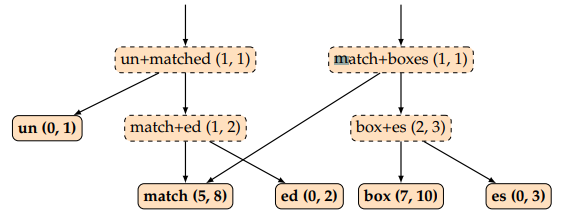
\includegraphics[width=7.2cm, height=3cm]{ComputationalLinguistics/Pictures/morph.png}
\end{center}

\end{frame}

\begin{frame}[fragile]{Morfessor}{Метрика}
$$precision = \frac{number\ of\ correct\ boundaries\ found}{total\ number\ of\ boundaries\ found}$$
$$recall = \frac{number\ of\ correct\ boundaries\ found}{total\ number\ of\ correct\ boundaries} $$
$$F = \frac{2 \cdot precision \cdot recall}{precision + recall}$$
Для английского примерно 0.77 в unsupervised и 0.86 в semi-supervised
\end{frame}

\subsection{Другие подходы}
\begin{frame}[fragile]{Другие подходы}
\begin{itemize}
    \item MORSE
    \item Seq2seq
\end{itemize}
\end{frame}

\appendix
\section<presentation>*{\appendixname}
\subsection<presentation>*{Useful links}

\begin{frame}[allowframebreaks]
  \frametitle<presentation>{Полезные ссылки}
    
  \begin{thebibliography}{10}
{
  \beamertemplatearticlebibitems
  % Start with overview books.
  
  \bibitem{morfessor1}
  \texttt{Morfessor2.0:Python Implementation and Extensions for Morfessor Baseline}
  \newblock \href{https://aaltodoc.aalto.fi/bitstream/handle/123456789/11836/isbn9789526055015.pdf}{\texttt{https://bit.ly/2QAzWtW}}
 
\bibitem{morfessor2}
  \texttt{Morfessor 2.0: Toolkit for statistical morphological segmentation}
  \newblock \href{https://www.aclweb.org/anthology/E14-2006}{\texttt{https://www.aclweb.org/anthology/E14-2006}}
  
\bibitem{morse}
  \texttt{MORSE: Semantic-ally Drive-n MORpheme SEgment-er}
  \newblock \href{https://arxiv.org/abs/1702.02212}{\texttt{https://arxiv.org/abs/1702.02212}}
  
\bibitem{dialog1}
  \texttt{Morphological Segmentation with Sequence to Sequence Neural Network}
  \newblock \href{http://www.dialog-21.ru/media/4287/arefyevnv.pdf}{\texttt{http://www.dialog-21.ru/media/4287/arefyevnv.pdf}}
  
  \bibitem{dialog2}
  \texttt{Use of morphology in distributional word embedding models:
Russian language case}
  \newblock \href{http://www.dialog-21.ru/media/4260/sadov\_kutuzov.pdf}{\texttt{http://www.dialog-21.ru/media/4260/sadov\_kutuzov.pdf}}

\beamertemplateonlinebibitems
\bibitem{morphessor-demo}
  \texttt{Morphessor 2.0 demo}
  \newblock \href{https://asr.aalto.fi/morfessordemo/}{\texttt{https://asr.aalto.fi/morfessordemo/}}

\bibitem{github1}
  \texttt{Morphessor 2.0}
  \newblock \href{https://github.com/aalto-speech/morfessor}{\texttt{https://github.com/aalto-speech/morfessor}}
  
  \bibitem{github2}
  \texttt{morpheme\_seq2seq}
  \newblock \href{https://github.com/kpopov94/morpheme\_seq2seq}{\texttt{https://github.com/kpopov94/morpheme\_seq2seq}}
  
\bibitem{github3}
  \texttt{XMorphy}
  \newblock \href{https://github.com/alesapin/XMorphy}{\texttt{https://github.com/alesapin/XMorphy}}
  
  
  
}

    
  \end{thebibliography}
\end{frame}

\end{document}


